
%%%%%%%%%%%%%%%%%%%%%%% file typeinst.tex %%%%%%%%%%%%%%%%%%%%%%%%%
%
% This is the LaTeX source for the instructions to authors using
% the LaTeX document class 'llncs.cls' for contributions to
% the Lecture Notes in Computer Sciences series.
% http://www.springer.com/lncs       Springer Heidelberg 2006/05/04
%
% It may be used as a template for your own input - copy it
% to a new file with a new name and use it as the basis
% for your article.
%
% NB: the document class 'llncs' has its own and detailed documentation, see
% ftp://ftp.springer.de/data/pubftp/pub/tex/latex/llncs/latex2e/llncsdoc.pdf
%
%%%%%%%%%%%%%%%%%%%%%%%%%%%%%%%%%%%%%%%%%%%%%%%%%%%%%%%%%%%%%%%%%%%


\documentclass[runningheads,a4paper]{llncs}

\setcounter{tocdepth}{3}
\usepackage{graphicx}
% For citations
\usepackage{natbib}
\usepackage{amsmath,amsfonts,amscd,amssymb}
\usepackage{dsfont}
\renewcommand{\vec}[1]{\mathbf{#1}}
\usepackage{hyperref}
\DeclareMathOperator*{\argmax}{argmax}
\DeclareMathOperator*{\argmin}{argmin}
\DeclareMathOperator*{\Corr}{Corr}
\newcommand{\R}{\mathds{R}}
\usepackage{multicol}
\usepackage{multirow}
\usepackage{pbox}
\usepackage{url}
\urldef{\mailsa}\path|{felix.biessmann,|
\newcommand{\keywords}[1]{\par\addvspace\baselineskip
\noindent\keywordname\enspace\ignorespaces#1}

\begin{document}

\mainmatter  % start of an individual contribution

% first the title is needed
\title{Automating Political Bias Prediction}

% a short form should be given in case it is too long for the running head
\titlerunning{Political Bias Prediction}

% the name(s) of the author(s) follow(s) next
%
% NB: Chinese authors should write their first names(s) in front of
% their surnames. This ensures that the names appear correctly in
% the running heads and the author index.
%
\author{
%Felix Bie\ss{}mann%
\thanks{}
%
\authorrunning{Political Bias Prediction}}
% (feature abused for this document to repeat the title also on left hand pages)

% the affiliations are given next; don't give your e-mail address
% unless you accept that it will be published
%\institute{
%\mailsa\\
%\mailsb\\
%\mailsc\\
%\url{http://www.springer.com/lncs}}

%
% NB: a more complex sample for affiliations and the mapping to the
% corresponding authors can be found in the file "llncs.dem"
% (search for the string "\mainmatter" where a contribution starts).
% "llncs.dem" accompanies the document class "llncs.cls".
%

\toctitle{Political Bias Prediction}
\tocauthor{}
\maketitle

\begin{abstract} 
Every day media generate large amounts of text. An unbiased view on what media report on requires an understanding of the political bias of media content. Assistive technology for estimating the political bias of texts can be helpful in this context. This study proposes a simple statistical learning approach to predict political bias from text. Standard text features extracted from speeches and manifestos of political parties are used to predict political bias in terms of political party affiliation and in terms of political views. Results indicate that political bias can be predicted with well above chance accuracy. Mistakes of the model can be interpreted with respect to changes of policies of political actors. Two approaches are presented to make the results more interpretable: a) discriminative text features are related to the political orientation of a party and b) sentiment features of texts are correlated with a measure of political power. Political power appears to be strongly correlated with positive sentiment of a text. To highlight some potential use cases a web application shows how the model can be used for texts for which the political bias is not clear such as news articles.
\end{abstract} 

\section{Introduction}
\label{sec:intro}
%
Modern media generate a large amount of content at an ever increasing rate. Keeping an unbiased view on what media report on requires to understand the political bias of texts. In many cases it is obvious which political bias an author has. In other cases some expertise is required to judge the political bias of a text. 
%
When dealing with large amounts of text however there are simply not enough experts to examine all possible sources and publications. Assistive technology can help in this context to try and obtain a more unbiased sample of information. \\

Ideally one would choose for each topic a sample of reports from the entire political spectrum in order to form an unbiased opinion. But ordering media content with respect to the political spectrum at scale requires automated prediction of political bias. And determining a political spectrum that goes beyond the two dimensional left-right scheme is difficult in itself. The aim of this study is to provide some empirical evidence indicating that leveraging some valuable open data sources political bias prediction is possible with above chance accuracy. \\


Automated predictions of political bias can be problematic for ethical reasons. One trusts political experts, as they will take responsibility for what they say about a text, and they can explain their decisions. This is a key difference to many statistical learning approaches. Not only is the responsibility question not entirely clear, it can also be difficult to interpret some of the decisions. In order to validate the predictions of the models we devise two strategies that allow for better interpretations of the models. First we are looking at univariate measures of how discriminative the features are that the model uses. This somewhat allows to relate the political texts to the kind of information that political experts use, too. Second we use sentiment analysis to investigate whether this aspect of language also has discriminatory power. \\


In the following \autoref{sec:data} gives an overview of data acquisition and preprocessing, \autoref{sec:model} presents the model, in \autoref{sec:results} the results are discussed and \autoref{sec:conclusion} concludes with some interpretations of the results and future research directions. 

\section{Data Sets and Feature Extraction}\label{sec:data}
%
We used publicly available data sets of german political texts and standard libraries for processing the text. The following sections describe the details of data acquisition and feature extraction. 

\subsection{Data}
We obtained annotated political text data from sources a) the discussions and speeches held in the german parliament ({\em Bundestag}) and b) all manifesto texts from parties running for election in the german parliament in the current 18th and the last, 17th, legislation period.

\paragraph{Parliament discussion data} Parliament texts are annotated with the respective party label, which we take here as a proxy of political bias. The texts of parliament protocols are available through the website of the german bundestag\footnote{\url{https://www.bundestag.de/protokolle}}, we used an open source API to that data to query the data in cleaned and structured format\footnote{\url{https://github.com/bundestag}}. This API returns for each speech the speaker and its party affiliation. In total we obtained 22784 speeches for the 17th legislative period and 11317 speeches for the 18th period, queried until March 2016. 

\paragraph{Party manifesto data}
For party manifestos we also use an openly accessible API provided by the Wissenschaftszentrum Berlin (WZB). The API is released as part of the {\em Manifestoproject} \cite{manifesto}. The data released in this project comprises the complete manifestos for each party that ran for election enriched with annotations by political experts. Each sentence (in some cases also parts of sentences) are labels with one of 56 political labels. Examples of these labels are {\em pro/contra protectionism, decentralism, centralism, pro/contra welfare, ...}. The set of labels was developed by political scientists at the WZB and released for public use. We obtained all manifestos of parties that were running for election in this and the last legislative period. In total this resulted in 29451 political statements that had two types of labels, for one we stored the party affiliation of each political statement. This party affiliation label was used to evaluate the party evaluation classifiers trained on the parliament speeches. For this purpose we constrained the data to only those parties that were elected into the parliament. Next to the party affiliation we were mainly interested in the political view labels annotated by human experts. For the analyses based on political view labels we considered all parties, also those that did not make it into the parliament. 

\subsection{Bag-of-Words Vectorization}\label{sec:bow-vectorization}
First each data set was segmented into semantic units; in the case of parliament discussions this were the speeches, in the case of the party manifesto data semantic units were the sentences or sentence parts associated with one of the 56 political view labels.  Parliament speeches were often interrupted; in this case each uninterrupted part of a speech was considered a semantic unit. Strings of each semantic unit were tokenized and transformed into bag-of-word vectors as implemented in scikit-learn \cite{scikit-learn}. The general idea of bag-of-words vectors is to simply count occurences of words (or word sequences, also called {\em n-grams}) for each data point. A data point is usually a documents, here it is the semantic units of parliament speeches and manifesto sentences, respectively. The text of each semantic unit is transformed into a vector $\vec{x}\in\mathds{R}^d$ where $d$ is the size of our dictionary; the $w$th entry of $\vec{x}$ contains the (normalized) count of the $w$th word (or sequence of words) in our dictionary. We tried several options for vectorizing the speeches, including term-frequency-inverse-document-frequency normalisation using n-gram patterns up to size $n=3$ and several cutoffs for discarding too frequent and too infrequent words. All of these hyperparameters were subjected to hyperparameter optimization as explained in \autoref{sec:crossvalidation}. 


\section{Classification Model and Training Procedure}\label{sec:model}
We used a multinomial logistic regression model in order to classify bag-of-words feature vectors. Let $y\in\{1,2,\dots,K\}$ be the true  label (party affiliation or political view, see \autoref{sec:data}), where $K$ is the total number of labels and $\vec{W}=[\vec{w}_1,\dots,\vec{w}_K]\in\R^{d\times K}$ is the concatenation of the weight vectors $\vec{w}_k$ associated with the $k$th party then 
\begin{eqnarray}\label{eq:logreg_multiclass}
p(y=k|\vec{x},\vec{W}) = &\frac{e^{z_k}}{\sum_{j=1}^K e^{z_j}} \qquad \textrm{with }  z_k=&\vec{w}_k^{\top}\vec{x} \\\nonumber
\end{eqnarray}
%
We estimated $\vec{W}$ using quasi-newton gradient descent. The optimization function was obtained by adding a penalization term to the negative log-likelihood of the multinomial logistic regression objective and the optimization hence found the $\vec{W}$ that minimized
\begin{equation}\label{eq:objective}
L(\vec{W}, \vec{x}, \gamma) = - \log{\frac{e^{z_k}}{\sum_{j=1}^K e^{z_j}}}+ \gamma \| \vec{W} \|_{F}
\end{equation}
Where $\|~\|_F$ denotes the Frobenius Norm and $\gamma$ is a regularization parameter controlling the complexity of the model. 
 We optimized the regularization parameter on a log-scaled grid from $10^{-4,\dots,4}$ and the regularization constant was adopted to reflect asymmetric class frequency distributions. The performance of the model was optimized using the classification accuracy, but we also report all other standard measures, precision ($TP / (FP + TP$), recall ($TP / (TP + FN)$) and f1-score ($2\times (Prec. \times Rec) / (Prec + Rec.)$). 

We considered three different classification problems: 
\begin{enumerate}
\item {\bf Classification of party affiliation} (5 class problem for the 17th legislation period, 4 class problem for the 18th legislation period)
\item {\bf Classification of government membership} (binary problem)
\item {\bf Classification of political views} as expressed by the political codes of the manifestoproject (56 class problem)
\end{enumerate}

For each of first two problems, party affiliation and government membership prediction, we trained classifiers on the parliament speeches. For the third problem we trained only on the manifesto data as only for those the political view labels were available. 

\subsection{Optimisation of Model Parameters}\label{sec:crossvalidation}
The model pipeline contained a number of {\em hyperparameters} that we did not want to tune by hand. 
We first split the training data into a training data set that was used for optimization of hyperparameters and an held-out test data set for evaluating how well the model performs on in-domain data; next to the in-domain test data, we also used out-of domain data wherever possible in order to evaluate how well the model would generalize to text domains that the model has not seen during training. The test data for hyperparameter optimization was 10\% of the entire training data. Hyperparameters were optimized using grid search and 3-fold cross-validation within the training set only: Within the training set a cross-validation split was made to obtain train/test data for the grid search and for each setting of hyperparameters the entire pipeline was trained and evaluated -- no data from the in-domain evaluation data or the out-of-domain evaluation data were used for hyperparameter optimization. For the best setting of all hyperparameters, we trained the pipeline again on all training data and evaluated it on both evaluation data sets. For party affiliation prediction and government membership prediction the training and test set were 90\% and 10\%, respectively, of all data in a legislative period. Out-of-domain evaluation data were the texts from party manifestos. For the political view prediction setting we first split all labeled manifesto sentences in both legislative periods into a training/test and evaluation set of 90\% (train/test) and 10\% (evaluation), then we split the train/test part again with a 90\%/10\% ratio for training/evaluating of the hyperparameters. 

\subsection{Sentiment analysis}\label{sec:sentiment_analysis_methods}
We used a publicly available key word list to extract sentiments from the text subjected to classification \cite{remquahey2010}. The sentiment index used for attributing positive or negative sentiment to a text was computed  as the cosine similarity between bag-of-word vectors $\vec{x}\in\R^d$ and sentiment vector $\vec{s}\in\R^d$ which was constructed by simply taking the values from the sentiment dictionary. 

\subsection{Analysing bag-of-words features}
In order to get  better picture of which features contribute to the classification we computed correlation coefficients between each word and each party. Often linear models are interpreted by just looking at the weights of the model. Since the text features are obtained from real data and thus correlated we cannot inspect the model by interpreting the coefficients of $\vec{W}$, see e.g. \cite{Haufe2013}.  We thus only use univariate correlation to investigate how discriminative features are. The words corresponding to the top positive and negative correlations are shown in section \autoref{sec:word_party_correlations}.

\section{Results}\label{sec:results}

The following sections provide an overview of the results for both types of political bias prediction tasks, party affiliation and political view. Some interpretations of discriminative features are given one section will highlight a finding on the correlation of political power and positive sentiment of political texts. 

\subsection{Predicting political party affiliation}
The results for the political party affiliation prediction on held-out parliament data and on evaluation data are shown in \autoref{tab:results_17} for the 17th Bundestag and in \autoref{tab:results_18} for the 18th Bundestag, respectively. 
Shown are the evaluation results for in-domain data (held-out parliament speech texts) as well as the out-of-domain data results obtained from testing the models on the texts extracted from party manifestos. When looking at predicting party affiliation from text data from the same domain that was used for training precision and recall values of above 0.6 are obtained. For out-of domain data the models yield significantly lower precision and recall values between 0.3 and 0.4.  \\

\begin{table}[t]
\begin{center}
\begin{tabular}{lcccccccc}
& \multicolumn{4}{c}{\bf Held-out parliament speeches} & \multicolumn{4}{c}{\bf Party Manifestos}\\
    &         precision    &recall &  f1-score  & N    &         precision    &recall &  f1-score  & N\\
\hline \hline
       cducsu   &    0.62  &    0.81  &    0.70  &     706&0.26    &  0.58   &   0.36    &  2030\\
        fdp    &   0.70   &   0.37  &    0.49    &   331&0.38   &   0.28    &  0.33   &   2319\\
     gruene &      0.59  &    0.40   &   0.48   &    298&0.47  &    0.20   &   0.28 &     3747\\
      linke    &   0.71   &   0.61  &    0.65    &   338&0.30   &   0.47   &   0.37    &  1701\\
        spd   &    0.60   &   0.69  &    0.65   &    606&0.26   &   0.16   &   0.20  &    2278\\
\hline
avg / total &      0.64   &   0.63   &   0.62    &  2279 &0.35    &  0.31 &     0.30   &  12075
%
\end{tabular}
\end{center}
\caption{
\label{tab:results_17}
Classification performance on the party affiliation prediction problem for data from the 17th legislative period on test set and evaluation set, respectively.
}
\end{table}

\begin{table}[t]
\begin{center}
\begin{tabular}{lcccccccc}
& \multicolumn{4}{c}{\bf Held-out parliament speeches} & \multicolumn{4}{c}{\bf Party Manifestos}\\
    &         precision    &recall &  f1-score  & N    &         precision    &recall &  f1-score  & N\\
\hline \hline
    cducsu    &   0.66   &   0.82   &   0.73    &   456 & 0.32  &    0.64  &    0.43    &  2983\\
     gruene   &    0.68    &  0.54   &   0.60    &   173   &0.59   &   0.15   &   0.23   &   5674\\
      linke     &  0.77  &    0.58    &  0.66    &   173 & 0.36   &   0.48   &   0.41   &   2555\\
        spd     &  0.60  &    0.54   &   0.57    &   330 & 0.26 &     0.31   &   0.28     & 2989\\
\hline
avg / total    &   0.66  &    0.66  &    0.65   &   1132&  0.42 &     0.34  &    0.32&     14201\\
%
\end{tabular}
\end{center}
\caption{
\label{tab:results_18}
Classification performance on the party affiliation prediction problem for data from the 18th legislative period on test set and evaluation set, respectively. 
}
\end{table}


In order to investigate the errors the models made we extracted confusion matrices for the predictions on the out-of-domain evaluation data, the manifesto data. So the model, trained on party speeches in the parliament was tested on the texts parties published before the elections in order to get elected. One example in \autoref{tab:confusion} shows that these mistakes the model makes can give valuable insights into the changes in policy a party decides to make. The green party was promoting policies for renewable energy and agains nuclear energy in their manifestos prior to both legislative periods. When training a classifier on what representatives in the parliament say however, the statements of the green party are more often predicted to be from the conservative government than from the party that originally promoted these green ideas. This effect is also reflected in the precision values on out-of-domain data: The green party has the highest precision values by a large margin in both legislation periods, indicating that there is a relatively high true-positive rate. A similar effect was can be observed with the social democratic party (SPD): Evaluating the parliament classifier on manifestos it seems that a significant amount of speeches get classified as conservative government while being from the SPD. \\

Next to the party affiliation we also predicted whether or not a text is from a party that belonged to a given governing coalition of the Bundestag. In \autoref{tab:results_binary_17} and \autoref{tab:results_binary_18} the results are shown for the 17th and the 18th Bundestag, respectively. While the in-domain evaluation precision and recall values are much better in this case, reaching values close to 0.9, the out-of-domain evaluation drops again to values between 0.6 and 0.7. 

% Confusion matrix
\begin{table}[t]\label{tab:conf_mat_four_class}
\begin{tabular}{lcc|ccccc}
 \multicolumn{8}{c}{\bf 17th Bundestag}\\
 \\
&&& \multicolumn{5}{c}{Predicted}\\
&&& cducsu & fdp& gruene& linke& spd\\
\hline
\multirow{5}{*}{\rotatebox{90}{\pbox{3cm}{\centering True}}}& &cducsu &1186 &289& 178& 198& 179\\
&&fdp &882& 658& 236& 329& 214\\
&&gruene &1174& 404& 764& 941& 464\\
&&linke &388& 92& 214& 806& 201\\
&&spd &999& 268& 240& 398& 373\\
\end{tabular}
\quad
\begin{tabular}{lcc|cccc}
 \multicolumn{7}{c}{\bf 18th Bundestag}\\
 \vspace{1em}\\
&&& \multicolumn{4}{c}{Predicted}\\
&&& cducsu & gruene& linke& spd\\
\hline
\multirow{4}{*}{\rotatebox{90}{\pbox{4.7cm}{\centering True}}}&&cducsu&1912& 156& 331& 584\\
&&gruene&2092& 827& 1311& 1444\\
&&linke&596& 186& 1216& 557\\
&&spd&1284& 226& 563& 916\\
\end{tabular}
\vspace{1em}
\caption{\label{tab:confusion} Confusion matrices for predictions on evaluation data (party manifestos) for classifiers trained on parliament speeches for the 17th legislative period (left) and 18th legislative period (right); the most prominent effect is the high likelihood for a party to be taken as the strongest, governing party, cdu/csu. In particular the green party suffers from this effect: when trained on the speeches in the 18th Bundestag, 2092 statements out of the green party's manifesto were classified as belonging to the cducsu party. This can be interpreted as a change in policies of the conservative party cdu/csu towards the policies of the green party.}
\end{table}



\begin{table}[t]
\begin{center}
\begin{tabular}{lcccccccc}
& \multicolumn{4}{c}{\bf Held-out parliament speeches} & \multicolumn{4}{c}{\bf Party Manifestos}\\
    &         precision    &recall &  f1-score  & N    &         precision    &recall &  f1-score  & N\\
\hline \hline
government    &   0.83   &   0.84&      0.84     & 1037 & 0.49  &    0.59 &     0.54  &    4349\\
 opposition     &  0.86  &    0.86   &   0.86    &  1242 & 0.74 &     0.66  &    0.70   &   7726\\
\hline
avg / total   &    0.85 &     0.85 &     0.85  &    2279 & 0.65  &     0.63  &     0.64  &    12075\\

%
\end{tabular}
\end{center}
\caption{
\label{tab:results_binary_17}
Classification performance on the binary prediction problem in the 17th legislative period, categorizing speeches into government (FDP/CDU/CSU) and opposition (Linke, Gr\"une, SPD).
}
\end{table}

\begin{table}[t]
\begin{center}
\begin{tabular}{lcccccccc}
& \multicolumn{4}{c}{\bf Held-out parliament speeches} & \multicolumn{4}{c}{\bf Party Manifestos}\\
    &         precision    &recall &  f1-score  & N    &         precision    &recall &  f1-score  & N\\
\hline \hline
government   &    0.88  &    0.95    &  0.92   &    786   &0.52   &   0.66 &     0.58  &    5972\\
 opposition    &   0.86    &  0.71   &   0.78   &    346 & 0.69  &    0.56    &  0.62   &   8229\\
\hline
avg / total    &   0.88    &  0.88     & 0.87  &    1132 &  0.62   &   0.60    &  0.60 &    14201\\
%
\end{tabular}
\end{center}
\caption{
\label{tab:results_binary_18}
Classification performance on the binary prediction problem in the 18th legislative period, categorizing speeches into government (SDP/CDU/CSU) and opposition (Linke, Gr\"une).
}
\end{table}


\subsection{Predicting political views}

\begin{table}[t]
\begin{center}
\begin{tabular}{lrrrr}
    &         precision    &recall &  f1-score  & N\\
\hline\hline
test set    &  0.48   &   0.47  &    0.47  &    2651\\
evaluation set    &  0.47    &  0.46 &     0.46 &     2946\\
%
\end{tabular}
\end{center}
\caption{
\label{tab:results_avg_political_view}
Classification performance on the 56 class prediction problem of political views, see \autoref{sec:data}.
}
\end{table}

\subsection{Speech sentiment correlates with political power}\label{sec:sentiment_result}
In order to investigate the features that give rise to the classifiers' performance the bag-of-words features were analysed with respect to their sentiment. The average sentiment of each political party is shown in \autoref{fig:party_sentiments} for the two legislative periods under investigation. While the methodology used for estimating the sentiment (see \autoref{sec:sentiment_analysis_methods}) is simple and limited to a one dimensional spectrum of sentiment, it can yield some insight into the emotional content of a speech. High values indicate more pronounced usage of positive words, whereas negative values indicate more pronounced usage of words associated with negative emotional content. 

The results show an interesting relationship between political power and sentiment. Political power was evaluated in two ways: a) in terms of the number of seats a party has and b) in terms of membership of the government. Correlating either of these two proxies of political power with the mean sentiment of a party shows a strong positive correlation between speech sentiment and political power. This pattern is evident from the barplot in \autoref{fig:party_sentiments} and in \autoref{tab:sentiments}: In the current Bundestag, government membership correlates with positive sentiment with a correlation coefficient of 0.98 and the number of seats correlates with 0.89. 

Note that there is one party, the social democrats (SPD), which have a large number of seats and were in the opposition in the 17th Bundestag and member of the government in the 18th Bundestag: The average sentiment of this party switched sign from negative to positive when they joined the government, indicating that positive sentiment is a strong indicator of government membership of affiliation when analysing a text. 

\begin{figure}
\begin{center}
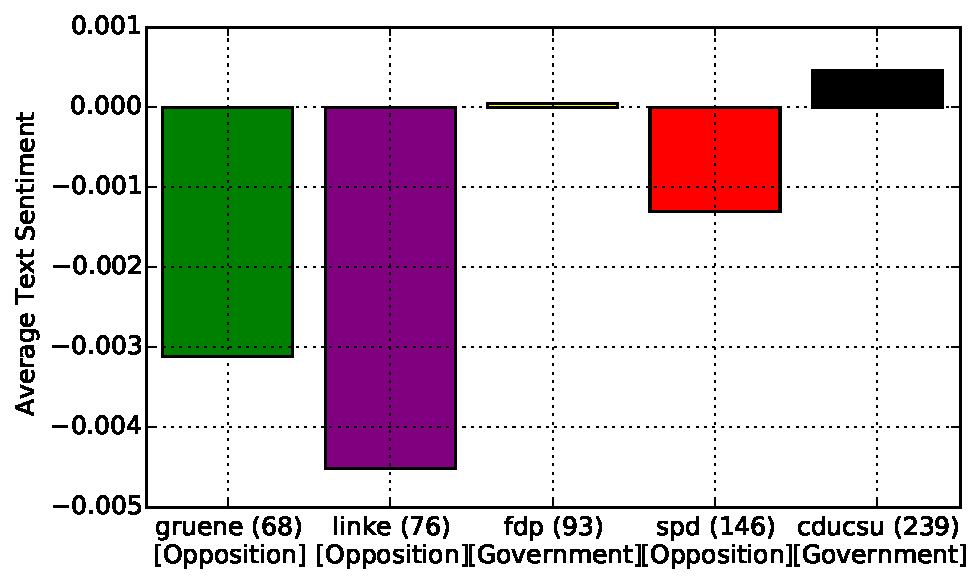
\includegraphics[width=6cm]{images/party-sentiments-17.pdf}  \hfill 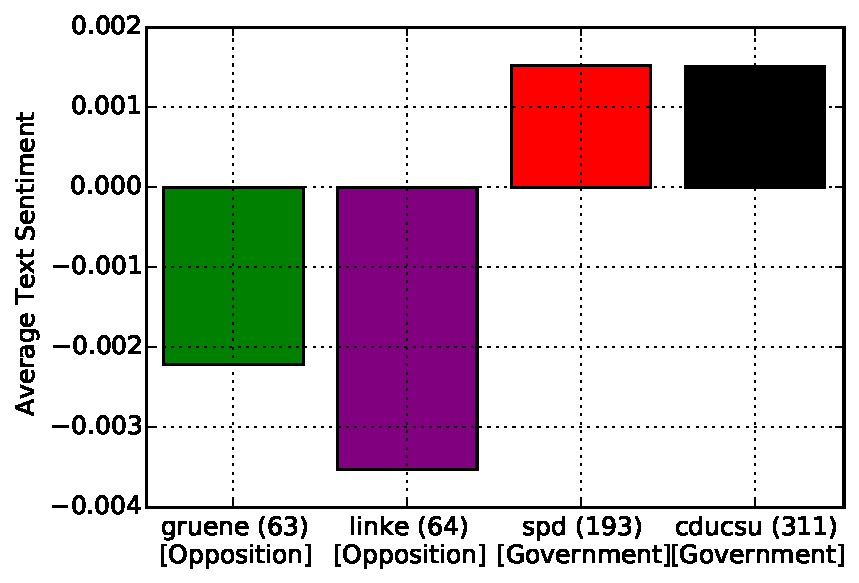
\includegraphics[width=6cm]{images/party-sentiments-18.pdf} 
%
\end{center}
\caption{
\label{fig:party_sentiments}
Speech sentiments computed for speeches of each party; parties are ordered according to political power measured in number of seats in the parliament from left to right. The more political power a party has, the more positive the speech content is. Note that while the SPD (red) was in the opposition in the 17th Bundestag it became part of the government in the 18th Bundestag: their seats in the parliament increased and the average sentiment of their speeches switched sign from negative to overall positive sentiment.
}
\end{figure}

\begin{table}[t]
\begin{center}
\begin{tabular}{lcc}
   Sentiment vs. &          Gov. Member    &  Seats\\
\hline\hline
17th Bundestag    &  0.84 & 0.70\\
18th Bundestag   &  0.98 & 0.89\\
%
\end{tabular}
\end{center}
\caption{
\label{tab:sentiments}
Correlation coefficient between average sentiment of political speeches of a party in the german bundestag with two measures of their political power, a) their membership in the government and b) with the number of seats that party occupies in the parliament. Shown are correlations for the 17th legislative period and the (ongoing) 18th legislative period.
}
\end{table}



\subsection{Correlations between words and parties}\label{sec:word_party_correlations}

\autoref{fig:party_word_correlations} shows the correlations of individual words and each party. We plotted the top 20 words for each sign, i.e. the 20 words with the strongest positive and negative correlations for each party, respectively. While the correlations do indicate that there are -- despite extensive and careful cleaning procedures -- still words with strong correlations in the top words, we conjecture that at least some of these words do have some discriminatory power, even if they do not refer to political views. Below we list some examples, but the most prominent is probably: the opposition often addresses the government in their speeches, the govermental parties do that less often. This is reflected in the frequency of the usage of words that refer to members of the government or ministers. But among the often used and avoided words we also find words that refer to actual political content. Thus we hypothesize that to some extent these correlation coefficients can give hints as to what the bag-of-words histogram representation into which we transformed the speeches are related to the actual content of the speeches. In the following we give some examples of words that appear to be preferentially used or avoided by each respective party. Even though interpretations of these quantitative results are somewhat invalid, as they neglect the context in which these words were mentioned, we find some interesting patterns. 

\begin{figure}
\begin{center}
%\includegraphics[width=3.5cm]{party_word_correlations-linke.pdf} 
%\includegraphics[width=3.1cm]{party_word_correlations-gruene.pdf} 
%\includegraphics[width=3.45cm]{party_word_correlations-spd.pdf} 
%\includegraphics[width=3.65cm]{party_word_correlations-cdu.pdf}
%
\end{center}
\caption{
\label{fig:party_word_correlations}
Correlations between words and party for parliament speeches. }
\end{figure}

\subsection{An example web application}
We implemented an example web application that downloads regularly all articles from major german news paper websites\footnote{\url{http://www.spiegel.de/politik}, \url{http://www.faz.net/aktuell/politik}, \url{http://www.welt.de/politik}, \url{http://www.sueddeutsche.de/politik}, \url{http://www.zeit.de/politik}}, applies some simple topic modelling to them and assigns articles to a topic and predicts the political view of an article using the manifesto code classifier trained on all party manifestos. Within each topic it is then possible to get an order (from left to right) overview of the opinions on that topic. An example of one topic that emerged on March 31st is shown in \autoref{fig:fipi}. The demo is live and running\footnote{\url{http://to-be-included-in-camera-ready-version.com}} and the code is open sourced an available on git-hub\footnote{\url{http://to-be-included-in-camera-ready-version.com}}.
\begin{figure}
\begin{center}
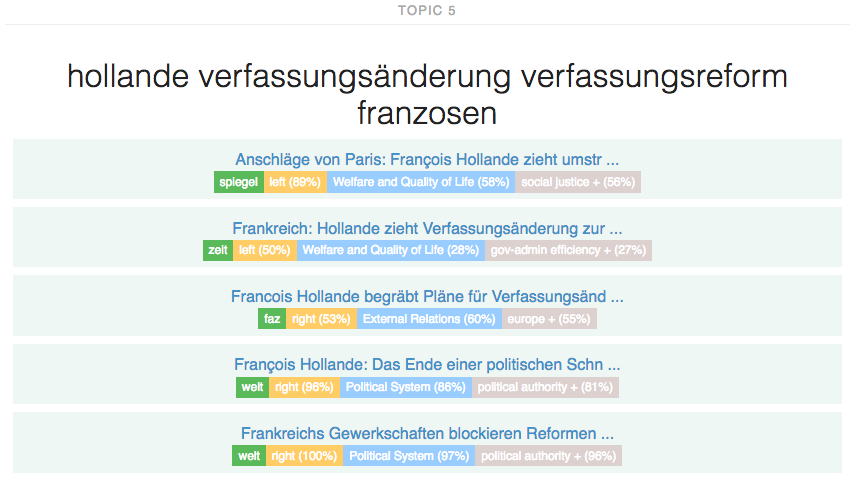
\includegraphics[width=10cm]{images/fipi-screenshot}
%
\end{center}
\caption{
\label{fig:fipi}
A screen shot of an example web application using the political view prediction combined with topic modelling to provide a heterogeneous overview of a topic. }
\end{figure}


\section{Conclusions, Limitations and Outlook}\label{sec:conclusion}
The goal of this study was to present a simple approach for automating political bias prediction and to quantify how well this is possible. The results of these experiments show that automated political bias prediction is possible with above chance accuracy. Moreover there are some interesting aspects of these analyses that could be interesting for social science researchers, too.

For one the misclassifications of a model can be related to the changes in policy of a party. This can be helpful to quantitatively back up such a change in policy with more than just anecdotal evidence from single texts. Second analysing the word-party correlations shows some discriminative words that are also used by the classifier to determine political bias. This insight can be related to the political views of a party and allows for validation of the models by human experts. Third when correlating the sentiment of a speech with proxies of political power there is a strong and significant positive correlation between political power and positive sentiment. This supports the (probably trivial) intuition that if we read a text that has a positive opinion on what the party in power does, the author of the text is probably affiliated with those in power. While such an insight of something rather obvious in itself might not be very useful, the technology behind it is: Sentiment analysis, and in particular such a simple approach as used here, can be easily automated and scaled up to massive amounts of text data. Having established such a way of relating this aspect of media content to the political bias allows to automate political bias direction using the proxy of sentiments, which are a rather domain-independent measure. 

One of the main limitations of an automated political bias prediction system is the availability of training data. Every training data set that is publicly available has an inherent bias as it is taken from a different domain. This study tried to quantify the impact of this, but not in all settings we had out-of-domain data to quantify generalization performance across text domains. 
For the cases where we had evaluation data from two domains there was a pronounced shift in performance between in-domain evaluation set and out-of-domain evaluation set. This was to be expected, given that the texts are written for a different audience and in completely different styles. This results in quite some non-stationarities or covariate shifts between the in-domain and out-of-domain evaluation data. Another important issue was that the semantic units in the case of the out-of-domain data were of much shorter length (often just parts of a sentence) and hence much noisier than the in-domain evaluation data. \\

Taken together the results show that when training on one domain and evaluating on an entirely different domain one can still obtain above chance performance, even though there is a significant drop in performance. The generalization performance across domains will be an important topic of future research. The aim of this study was mainly to assess the impact of this effect, but if the goal is to minimize the generalization performance the simplest solution, next to more complicated approaches from semisupervised learning, non-stationary methods or covariate shift approaches, is to simply include data from different -- possibly very heterogeneous -- domains in the training data set.  A popular approach is to integrate data from social networks such as Facebook, as advocated for instance in \cite{Arzheimer2016}. \\

All data sets used in this study were publicly available, all code for experiments and the live web application can be found online \cite{fipi, fipidemo}.
%-- in fact even the very definition of a spectrum could be considered a difficult problem. The aim of this study is to investigate

\subsection*{Acknowledgements}
This study would not have been possible without the open data initiatives behind the code and projects that led to the publicly available data sets and APIs described in \autoref{sec:data}.
%
\small{
\bibliographystyle{plain}
\bibliography{political_bias_prediction} 
}


\end{document}
